\section{Variables Aleatorias Unidimensionales}
\subsection{Concepto de Variable Aleatoria}
\begin{itemize}[label=\color{red}\textbullet, leftmargin=*]
	\item \color{lightblue}Definición
\end{itemize}
Sea $(\Omega,\mathcal{S}, P)$ espacio de probabilidad. Llamaremos variable aleatoria a una aplicación $x:\Omega\longrightarrow\R$ que a cada resultado del espacio muestral le asocia un número de la recta real y tal que \[ x^{-1}\left((-\infty,x]\right)=\{w\in\Omega:x(w)\le x\}\in\mathcal{S} \]
\begin{wrapfigure}{r}{0.5\textwidth}
	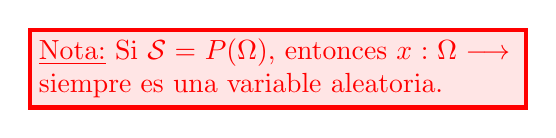
\begin{tikzpicture}
		\node[red, draw=red, fill=red!10, line width=1.5, text width=0.5\textwidth] {\underline{Nota:} Si $\mathcal{S}=P(\Omega)$, entonces $x:\Omega\longrightarrow\R$ siempre es una variable aleatoria.};
	\end{tikzpicture}
\end{wrapfigure}

\Ej

$X=$"Nº de unidades defectuosas en un lote de 100 unidades" es una variable aleatoria \lb{discreta}.

$X=$"Concentración de $CO_2$ en el interior de la clase" es una variable aleatoria \lb{continua}.\\
Las variables aleatorias se denotan con letras mayúsculas, las últimas del abecedario: $X,Y,Z$
\subsection{Función de distribución}
\begin{itemize}[label=\color{red}\textbullet, leftmargin=*]
	\item \color{lightblue}Definición
\end{itemize}
Sea $X:\Omega\longrightarrow\R$ una variable aleatoria llamaremos \lb{función de distribución} de $X$ a $F_X:R\longrightarrow\R$. \[ x\longrightarrow F_X(x)=P(X\le x)=P(X\in(-\infty,x]) \]
\begin{itemize}[label=\color{red}\textbullet, leftmargin=*]
	\item \color{lightblue}Propiedades
\end{itemize}
\begin{enumerate}[label=\color{lightblue}\arabic*)]
	\item $F_X$ es monótona creciente, linealmente dependiente, si $\underset{\lb{x,y\in\R}}{x<y}\Longrightarrow F_X(x)\le F_X(y)$
	\item $F_X$ es continua por la derecha, linealmente independiente, $\lim_{t\to x^+}F_X(t)=F_X(x)$
	\item $\lim_{x\to-\infty}F_X(x)=0,\:\lim_{x\to+\infty}F_X(x)=1$
\end{enumerate}
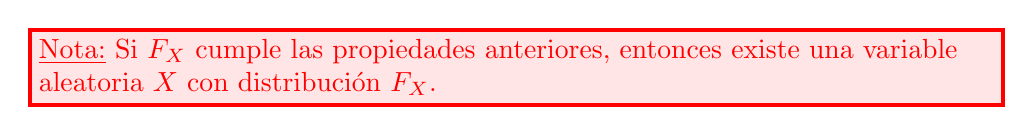
\begin{tikzpicture}
	\node[red, draw=red, fill=red!10, line width=1.5, text width=\textwidth] {\underline{Nota:} Si $F_X$ cumple las propiedades anteriores, entonces existe una variable aleatoria $X$ con distribución $F_X$.};
\end{tikzpicture}
\begin{itemize}[label=\color{red}\textbullet, leftmargin=*]
	\item \color{lightblue}Propiedades
\end{itemize}
Sea $F:\R\longrightarrow\R$ función de distribución. Entonces:
\begin{enumerate}[label=\color{lightblue}\arabic*)]
	\item $F(x)=P(X\le x)$
	\item $P(X<x)=P(X\in(-\infty, x))=F(X)=\lim_{t\to x}F(x)$
	\item $0\le F(x)\le1\:\forall x\in\R$
	\item $P(A<X\le b)=F(b)-F(a)$
	\item $P(a<X<b)=F(b^{-})-F(a)$
	\begin{center}
		\begin{tikzpicture}[scale=2]
			\draw (-3,0) -- (2,0);
			\draw[lightblue, decorate, decoration={zigzag}] (1,0) -- (-1,0);
			\draw[lightblue, decorate, decoration={zigzag}] (1,1) -- (-3,1);
			\draw[lightblue, decorate, decoration={zigzag}] (-1,0.5) -- (-3,0.5);
			\draw[lightblue] (-1,0) circle (0.05) node[below] {$a$};
			\filldraw[lightblue] (1,0) circle (0.05) node[below] {$b$};
			\filldraw[lightblue] (1,1) circle (0.05);
			\filldraw[lightblue] (-1,0.5) circle (0.05);
		\end{tikzpicture}
	\end{center}
	\item $P(X=a)=F(a)-F(a^-)$
\end{enumerate}
\begin{itemize}[label=\color{red}\textbullet, leftmargin=*]
	\item \color{lightblue}Definición
\end{itemize}
A la función $\overline{F}(x)=1-F(x)$ se le llama \lb{función de fiabilidad}. Tipos de variables aleatorias:
\begin{itemize}
	\item Discretas
	\item Continuas
\end{itemize}
\subsection{Variables Aleatorias Discretas}
\begin{itemize}[label=\color{red}\textbullet, leftmargin=*]
	\item \color{lightblue}Definición
\end{itemize}
Diremos que $X:\Omega\longrightarrow\R$ es una variable aleatoria discreta si toma un número finito o infinito numerable de valores con probabilidad no nula.

A los valores que toma $X$ se les llama rango de $X$ o soporte de $X$.\\
\begin{center}
	$\mathrm{Sop}(X)=\{x_1,x_2,\dots,x_n,\dots\}$ tales que $P(X=x_i)\neq0\:\forall1,2\dots,n,\dots$
\end{center}
\begin{itemize}[label=\color{red}\textbullet, leftmargin=*]
	\item \color{lightblue}Definición
\end{itemize}
Sea $X$ una variable aleatoria. Se llama \lb{función puntual de probabilidad} (f.p.p) a la función $p(x)=P(X=x)\:\forall x\in\R$
\begin{itemize}
	\item $p(x_i)=P(X=x_i)\:\forall x_i\in\sop(X)\longrightarrow$ Puntos del Soporte$(X)$
	\item $p(x)=P(X=x)\:\forall x\in\sop(X)\longrightarrow$ Puntos fuera del Soporte$(X)$
\end{itemize}
\begin{itemize}[label=\color{red}\textbullet, leftmargin=*]
	\item \color{lightblue}Propiedades
\end{itemize}
Sea $p(x)=P(X=x)$ \fpp de $X$. Entonces:
\begin{enumerate}[label=\color{lightblue}\arabic*)]
	\item $p(x)\ge0\:\forall x\in\R$
	\item $\underset{\lb{x_i\in\sop(X)}}{\sum p(x_i)}=1$
\end{enumerate}
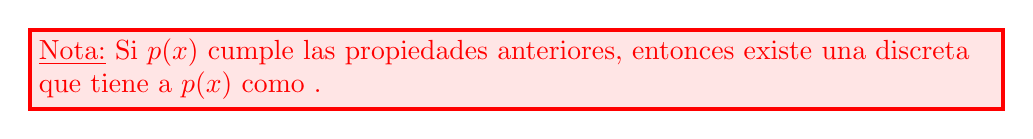
\begin{tikzpicture}
	\node[red, draw=red, fill=red!10, line width=1.5, text width=\textwidth] {\underline{Nota:} Si $p(x)$ cumple las propiedades anteriores, entonces existe una \va discreta que tiene a $p(x)$ como \fpp.};
\end{tikzpicture}
\begin{itemize}[label=\color{red}\textbullet, leftmargin=*]
	\item \color{lightblue}Propiedades
\end{itemize}
$p(x)$ \fpp de la \va discreta $X$ y sea $F(x)$ su función de distribución. Entonces:
\begin{enumerate}[label=\color{lightblue}\arabic*)]
	\item $F(x)=\underset{\lb{\begin{subarray}{c}
			x_i\in\sop(X)\\
			x_i\le x
	\end{subarray}}}{\sum p(x_i)}$
\item $P(a<X\le b)=\underset{\lb{\begin{subarray}{c}
			x_i\in(a,b]\\
			x_i\in\sop(X)\\
\end{subarray}}}{\sum p(x_i)}$
\item $P(X\in A)=\underset{\lb{\begin{subarray}{c}
		x_i\in\sop(X)\\
		x_i\in A
\end{subarray}}}{\sum p(x_i)}$
\end{enumerate}
\Ej

Representa la \fpp.

\begin{tikzpicture}
	\draw (-0.5,0) -- (4.5,0);
	\draw (0,-0.5) -- (0,2);
	\draw[lightblue, *-] (1,0.5) -- (1,0) node[below] {$x_1$};
	\draw[lightblue, *-] (2,1.5) -- (2,0) node[below] {$x_2$};
	\draw[lightblue, *-] (4,1) -- (4,0) node[below] {$x_n$};
	\node[lightblue, below] at (3,0) {$\cdots$};
	\draw[lightblue, dashed] (1,0.5) -- (0,0.5) node[left] {$P(x_1)$};
	\draw[lightblue, dashed] (4,1) -- (0,1) node[left] {$P(x_n)$};
	\draw[lightblue, dashed] (2,1.5) -- (0,1.5) node[left] {$P(x_2)$};
\end{tikzpicture}

\begin{tikzpicture}[scale=1.5]
	\node[above right] at (0,2.5) {$F(x)$: Función de distribución};
	\draw[lightblue, dashed] (0,0.25) node[left] {$P(x_1)$} -- (1,0.25) |- (0,0);
	\draw[lightblue, dashed] (0,1.25) node[left] {$P(x_1)+P(x_2)$} -- (2,1.25) |- (0,0);
	\draw[lightblue, dashed] (0,2) node[left] {$1$} -- (4,2) |- (0,0);
	\node[left, lightblue] at (0,1.75) {$\vdots$};
	\draw (-0.5,0) -- (5,0);
	\draw (0,-0.5) -- (0,2.5);
	\node[lightblue, below] at (3,0) {$\cdots$};
	\node[lightblue, below] at (1,0) {$x_1$};
	\node[lightblue, below] at (2,0) {$x_2$};
	\node[lightblue, below] at (4,0) {$x_n$};
	\draw[lightblue, line width=1.5] (-0.5,0) -- (1,0);
	\draw[lightblue, line width=1.5, [-] (1,0.25) -- (2,0.25);
	\draw[lightblue, line width=1.5, [-, rotate=180] (-2,-0.25) -- (-1,-0.25);
	\draw[lightblue, line width=1.5, [-] (2,1.25) -- (3,1.25);
	\draw[lightblue, line width=1.5, [-] (4,2) -- (5,2);
	\draw[lightblue, decorate, decoration={brace, amplitude=5pt}] (2,0.25) -- (2, 1.25) node[midway, left] {$P(x_2)$};
	\node[red, draw=red, fill=red!10, line width=1.5, text width=6cm] at (8, 1.5) {\underline{Nota:} Las \vas discretas tienen función de distribución escalonada, constante a otros en los puntos de soporte (o rango) y amplitud del salto igual a la probabilidad de dicho punto.};
\end{tikzpicture}
\subsection{Variables Aleatorias Continuas}
\begin{itemize}[label=\color{red}\textbullet, leftmargin=*]
	\item \color{lightblue}Definición
\end{itemize}
Llamaremos \lb{\va de tipo continuo} a las que tienen función de distribución continua.
\begin{itemize}[label=\color{red}\textbullet]
	\item \lb{Idea:} Las \vas continuas son las que toman valores en un intervalo de $\R$.
	\item \lb{Observación:} Si $X$ es una variable continua, entonces $P(X=x)=0\:\forall x\in\R$.
\end{itemize}
Vemos que $P(X=x)=F(x)-F(x^-)=0$
\begin{center}
	\begin{tikzpicture}
	\draw (-2,0) -- (1.2,0);
	\draw[lightblue] (1,0.1) -- (1,-0.1) node[below] {$x$};
	\draw[lightblue,[-] (1,1) -- (-2,1) node[above, midway] {$F(x)$};
	\draw[blue, (-] (1,0.5) -- (-2,0.5) node[below, midway] {$F(x^-)$};
	\end{tikzpicture}
\end{center}
En realidad nos concentraremos en \vas con función de distribución $F(x)$ derivable en "casi" todo punto, para así disponer de la función de densidad.
\begin{itemize}[label=\color{red}\textbullet, leftmargin=*]
	\item \color{lightblue}Definición
\end{itemize}
Diremos que $x:\Omega\longrightarrow\R$ es una \va de tipo \lb{absolutamente continuo} si existe $f:\R\longrightarrow\R^+$ no negativa e integrable tal que \[ F(x)=P(X\le x)=\int_{-\infty}^{x}f(t)\dt \]A la función $f(t)$ se le llama función de densidad y el soporte $X$ se define como $\sop(X)=\{x\in\R\text{ tal que }f(x)>0\}$
\begin{itemize}[label=\color{red}\textbullet, leftmargin=*]
	\item \color{lightblue}Propiedades
\end{itemize}
Sea $f:\R\longrightarrow\R$ función de densidad de la \va $x$. Entonces: 
\begin{enumerate}[label=\color{lightblue}\arabic*)]
	\item $f(t)\ge0\:\forall t\in\R\longrightarrow$ \lb{Demostración:} Por definición
	\item $\int_{-\infty}^{+\infty}f(t)=1\longrightarrow$ \lb{Demostración:} $\int_{-\infty}^{+\infty}f(t)=\lim_{x\to\infty}F(x)=1$
\end{enumerate}
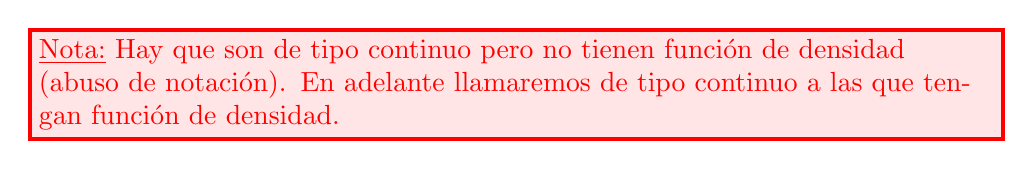
\begin{tikzpicture}
	\node[red, draw=red, fill=red!10, line width=1.5, text width=\textwidth] {\underline{Nota:} Hay \vas que son de tipo continuo pero no tienen función de densidad (abuso de notación). En adelante llamaremos \va de tipo continuo a las que tengan función de densidad.};
\end{tikzpicture}
\begin{itemize}[label=\color{red}\textbullet, leftmargin=*]
	\item \color{lightblue}Propiedades
\end{itemize}
Sea $x:\Omega\longrightarrow\R$ \va continua con función de densidad $f_X(x)$ y distribución $F(x)$. Entonces:
\begin{enumerate}[label=\color{lightblue}\arabic*)]
	\item $P(A<X<b)=P(a\le X< b)=P(a<X\le b)=P(a\le X\le b)=F(b)-F(a)=\int_a^bf_X(t)\dt.$
	\item $P(X\in A)=\int_Af_X(t)\dt$
	\item $F'(x)=f(x)$
	\item $F(x)=\int_{-\infty}^{x}f_x(t)\dt$
	\item $P(X=x)=0\:\forall x\in\R$
\end{enumerate}
\Ej

Si $F(x)=\begin{cases}
	0 & \text{si }x\le0\\
	x & \text{si }x\in[0,1)\\
	1 & \text{si }x\ge1
\end{cases}$ es función de distribución de la \va $X$, calcular su función de densidad $f_X(x)$.

$\bboxed{\begin{array}{l}
		f(x)=F'(x)=\begin{cases}
			1 & \text{si }x\in(0,1)\\
			0 & \text{en caso contrario}
		\end{cases}\\
		P(x>0.8)=1-F(0.8)=1-0.8=0.2
	\end{array}}$
\subsection{Cambios de variable}
\begin{itemize}[label=\color{red}\textbullet, leftmargin=*]
	\item \color{lightblue}Definición
\end{itemize}
Sea $X:\Omega\longrightarrow\R$ una \va y sea $g:\R\longrightarrow\R$ una función tal que la composición $Y=g(X):\underset{\lb{w\longrightarrow g(X(w))}}{\Omega\longrightarrow\R}$ es una \va. A la \va $Y$ se le llama cambio de variable sobre $X$.

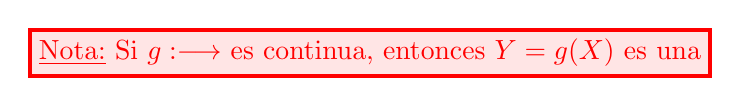
\begin{tikzpicture}
	\node[red, draw=red, fill=red!10, line width=1.5] {\underline{Nota:} Si $g:\R\longrightarrow\R$ es continua, entonces $Y=g(X)$ es una \va};
\end{tikzpicture}
\begin{itemize}[label=\color{red}\textbullet, leftmargin=*]
	\item \color{lightblue}Objetivos
\end{itemize}
\begin{enumerate}[label=\color{lightblue}\arabic*)]
	\item Obtener la función de distribución de $Y$ a partir de la función de distribución de $X$.
	
	\lb{¿Cómo lo haremos?}
	
	Realizando operaciones sobre la función de distribución.
	\item Obtener la \fpp de $Y$ en función de la \fpp de $X$
	
	\lb{¿Cómo lo haremos?}
	
	Operando directamente.
	\item Obtener la función de densidad de $Y$ a partir de la densidad de $Y$ a partir de la densidad de $X$.
	
	\lb{¿Cómo lo haremos?}
	
	Dos formas:
	\begin{enumerate}[label=\color{lightblue}\alph*)]
		\item Obtener la función de distribución y luego derivar.
		\item \lb{Teorema:} Sea $X:\Omega\longrightarrow\R$ \va continua con densidad $f_X(t)$ y soporte $\sop(X)\le I\subseteq\R$, sea $g:I\longrightarrow J\subseteq\R$ una \lb{biyección} e $Y=g(X)$ cambio de variable. Entonces: \[ \underset{\lb{\begin{subarray}{l}
					\text{función densidad}\\
					\text{de }Y
		\end{subarray}}}{f_Y(y)}=f_X\left(g^{-1}(y)\right)\cdot\left|\left(g^{-1}(y)\right)'\right| \]
	\end{enumerate}
\end{enumerate}
\Ej

Sea $X:\Omega\longrightarrow\R$ \va y $a,b\in\R$. Consideramos $Y=aX+b$. Observar que $Y$ es una \va porque $g(x)=aX+b$ es función continua. Obtener la función de distribución de $Y$ a partir de la de $X(F(X))$.

\begin{tikzpicture}
	\node[draw=lightblue, fill=lightblue!10, line width=1.5, text width=\textwidth] {
	$F_Y(y)=P(Y\le y)=P(aX+b\le y)=P(aX\le b-y)$\\
	\begin{itemize}[label=\color{red}\textbullet, leftmargin=*]
		\item \lb{Caso 1:} Si $a>0, F_Y(y)=P(aX\le b-y)=P\left(X\le\dfrac{b-y}{a}\right)=F_X\left(\dfrac{y-b}{a}\right)$
		\item \lb{Caso 2:} Si $a<0,F_Y(y)=P(aX\le b-y)=P\left(X\ge\dfrac{b-y}{a}\right)=\left\{\begin{tabular}{l}
			caso\\
			continuo
		\end{tabular}\right\}=1-F_X\left(\dfrac{y-b^-}{a}\right)$
	\item \lb{Caso 3:} Si $a=0,F_Y(y)=P(0\le y-b)=\begin{cases}
		1 & \text{si } y\ge b\\
		0 & \text{si }y<b
	\end{cases}$
\end{itemize}
	};
\end{tikzpicture} 

\Ej

Como en el ejemplo anterior, pero ahora suponemos $X$ \va discreta con \fpp $P_X(x)$. Considero $Y=aX+b$. Obtener la \fpp de $Y$ a partir de la de $X$.

\begin{tikzpicture}
	\node[draw=lightblue, fill=lightblue!10, line width=1.5, text width=\textwidth] {$P_X(y)=P(Y=y)=P(aX+b=y)$\\
	\begin{itemize}[label=\color{red}\textbullet, leftmargin=*]
		\item \lb{Caso 1:} $a\neq0,P_Y(y)=P(aX+b=y)=P\left(X=\dfrac{y-b}{a}\right)=P_X\left(\dfrac{y-b}{a}\right)$
		\item \lb{Caso 2:} $a=0,P_Y(y)=P(b=y)=\begin{cases}
			1 & \text{si }y=b\\
			0 & \text{si }y\neq b
		\end{cases}$
		\end{itemize}};
\end{tikzpicture}
\subsection{Esperanza, varianza y momentos de una variable aleatoria}
\begin{itemize}[label=\color{red}\textbullet, leftmargin=*]
	\item \color{lightblue}Definición
\end{itemize}
Sea $(\Omega,\mathcal{S},P)$ espacio probabilidad y sea $X:\Omega\longrightarrow\R$ una \va.
\begin{itemize}[label=$-$]
	\item Si $X$ es discreta con $\sop(X)=\{x_1,x_2,\dots,x_n,\dots\}$ y \fpp $p(x)$, se define la \lb{esperanza} o \lb{media} de $X$ como \begin{center}
		$\mu_X=E(x)=\underset{\lb{x_i\in\sop(X)}}{\sum x_i}\cdot p(x_i)=\begin{cases}
			0\cdot\dfrac{1}{2}+1\cdot\dfrac{1}{2}=\dfrac{1}{2}\\
			0\cdot\dfrac{1}{3}+1\cdot\dfrac{2}{3}=\dfrac{2}{3}
		\end{cases}$
	\end{center}
	\fcolorbox{red}{red!10}{\rc{\underline{Nota:} Para algunas \va no existe su media}}
	
	\item Si $X$ es continua con densidad $f(t)$, se define: \[ \mu_X=\int_{-\infty}^{+\infty}t\cdot f(t)\dt \]
\end{itemize}
\begin{itemize}[label=\color{red}\textbullet, leftmargin=*]
	\item \color{lightblue}Definición
\end{itemize}
Sea $X$ \va y $g:\R\longrightarrow\R$ función. Entonces:
\begin{itemize}[label=$-$]
	\item Si $X$ es discreta con $\sop(X)=\{x_1,x_2,\dots,x_n,\dots\}$ y \fpp $p(x)$, se define la \lb{esperanza} o \lb{media} de $X$ como \[ E\left(g(X)\right)=\bunderset{x_i\in\sop(X)}{\sum}g(x_i)\cdot p(x_i) \]
	\item Si $X$ es continua con densidad $f(t)$, se define: \[ E\left(g(X)\right)=\int_{-\infty}^{+\infty}g(t)\cdot f(t)\dt \]
\end{itemize}
\begin{itemize}[label=\color{red}\textbullet, leftmargin=*]
	\item \color{lightblue}Definición
\end{itemize}
Sea $X:\Omega\longrightarrow\R$ una \va
\begin{itemize}[label=$-$]
	\item Si $X$ es discreta con $\sop(X)=\{x_1,x_2,\dots,x_n,\dots\}$, se define la varianza de $X$ como \[ \var(X)=\sigma_X^2=\bunderset{x_i\in\sop(X)}{\sum}(x_i-\mu_X)^2\cdot p(x_i),\text{ con }\mu_X=E(x) \]
	\item Si $X$ es continua como antes, se define \[ \var(X)=\sigma_X^2=\int_{-\infty}^{+\infty}(t-\mu_X)^2\cdot f(t)\dt \]
\end{itemize}
\begin{itemize}[label=\color{red}\textbullet, leftmargin=*]
	\item \color{lightblue}Definición
\end{itemize}
$\sigma_X=\sqrt{\var(X)}$ desviación típica de $X$.
\begin{itemize}[label=\color{red}\textbullet, leftmargin=*]
	\item \color{lightblue}Propiedades
\end{itemize}
Sean $X:\Omega\longrightarrow\R$ e $Y:\Omega\longrightarrow\R$ \vas  ~y sean $a,b\in\R$. Entonces:
\begin{enumerate}[label=\color{lightblue}\arabic*)]
	\item $E(a)=a$
	\item $E(aX+b)=a\mu_X+b=a\cdot E(X)+b$
	\item $E(X+Y)=E(X)+E(Y)$
	\item Si $g(x)\le h(x)\:\forall x\longrightarrow E\left(f(x)\right)\le E\left(h(y)\right)$
	\item $\var(a)=0$
	\item $\var(aX+b)=a^2\var(X)$
	\item \fcolorbox{red}{red!10}{$\var(X)=E(x^2)-(E(x))^2$} \rc{!!}
	\item Si $X$ tiene media $\mu_X$ y varianza $\sigma_X^2$, entonces: \begin{center}
		$\dfrac{X-\mu_x}{\sigma}$ tiene media 0 y varianza 1
	\end{center}
\end{enumerate}
\begin{itemize}[label=\color{red}\textbullet, leftmargin=*]
	\item \color{lightblue}Definición
\end{itemize}
Sea $X:\Omega\longrightarrow\R$ \va llamaremos:
\begin{enumerate}[label=\color{lightblue}\alph*)]
	\item Momento ordinario o respecto al origen de orden $n$ a $\alpha_n=E(X^n)$
	\item Momento \lb{centrado} o respecto a la media de orden $n$ a 
	
	$\begin{array}{l}
		\mu_n=E\left((X-\mu_X)^n\right)\\
		\alpha_1=E(X)=\mu_X\text{ (media $X$)}\\
		\mu_2=\var(X)\text{ (varianza $X$)}
	\end{array}$
\end{enumerate}
\subsection{Desigualdades}
\begin{itemize}[label=\color{red}\textbullet, leftmargin=*]
	\item \color{lightblue}Teorema (Desigualdades de  Markov)
\end{itemize}
Sea $Z$ \va no negativa con media finita $E(Z)$\[ z:\Omega\longrightarrow\R \] y sea $a\in\R,a>0$. Entonces:\[ P(Z\ge a)\le\dfrac{E(z)}{a} \]
\begin{itemize}[label=\color{red}\textbullet, leftmargin=*]
	\item \color{lightblue}Demostración
\end{itemize}
Supongamos $Z$ \va discreta, con $\sop(Z)=\{z_1,z_2,\dots,z_n,\dots\}$ y \fpp $p(x)$.
\begin{enumerate}[label=\color{lightblue}\alph*)]
	\item $P(z\ge a)=a\cdot\bunderset{\begin{subarray}{l}
			x_i\in\sop(Z)\\
			x_i\ge a
	\end{subarray}}{\sum p(x_i)}=\bunderset{\begin{subarray}{l}
	x_i\in\sop(Z)\\
	x_i\ge a
\end{subarray}}{\sum a\cdot p(x_i)}\underset{\db{\begin{subarray}{l}
	\text{por ser}\\
	a\le x_i
\end{subarray}}}{\le}\bunderset{\begin{subarray}{l}
x_i\in\sop(Z)\\
x_i\ge a
\end{subarray}}{\sum x_i\cdot p(x_i)}\underset{\db{\begin{subarray}{l}
	\text{Hacemos términos}\\
	\text{no negativos}
\end{subarray}}}{\le}\bunderset{x_i\in\sop(Z)}{\sum x_i\cdot p(x_i)}=E(Z) $
\end{enumerate}

\begin{tikzpicture}
	\node[red, draw=red, fill=red!10, line width=1.5] {\underline{Nota:} Se puede demostrar de forma similar para caso continuo};
\end{tikzpicture}
\begin{itemize}[label=\color{red}\textbullet, leftmargin=*]
	\item \color{lightblue}Teorema (Desigualdad de Techebycher generalizada)
\end{itemize}
Sea $X$ \va con media finita y momento central de orden $n$ finito ($\mu_n$ finito). Sea $\varepsilon>0$, entonces:\[ \bboxed{P\left(|X-\mu\ge\varepsilon\right)\le\dfrac{E\left(|X-\mu|^n\right)}{\varepsilon^n}} \]
\begin{itemize}[label=\color{red}\textbullet, leftmargin=*]
	\item \color{lightblue}Demostración
\end{itemize}
Tomamos $z=|X-\mu|^n$ (\va no negativa) y $a=\varepsilon^n$ en el teorema anterior. Por tanto, aplicando \lb{Desigualdad de Markov} se tiene: \[ \bboxed{P\left(|X-\mu\ge\varepsilon\right)=P\left(|X-\mu|^n\ge \varepsilon^n\right)\le\dfrac{E\left(|X-\mu|^n\right)}{\varepsilon^n}} \]
\begin{itemize}[label=\color{red}\textbullet, leftmargin=*]
	\item \color{lightblue}Teorema (Desigualdad de Techebycher)
\end{itemize}
Sea $X:\Omega\longrightarrow\R$ \va (discreta o continua) con $\mu_X=E(X)$ y  $\sigma_X^2=\var(X)$ finitas, y sea $k>0$. Entonces:
\begin{enumerate}[label=\color{lightblue}\alph*)]
	\item $P(|X-\mu_X|\ge k\cdot \sigma_x)\le\dfrac{1}{k^2}$
	\item $P(|X-\mu_x|< k\cdot \sigma_x)\ge1-\dfrac{1}{k^2}$
\end{enumerate}
\begin{itemize}[label=\color{red}\textbullet, leftmargin=*]
	\item \color{lightblue}Demostración
\end{itemize}
\begin{enumerate}[label=\color{lightblue}(\alph*)]
	\item Tomamos $\varepsilon=k\cdot\sigma_X$ en la desigualdad de Techebycher generalizada, y tomamos $\varepsilon>0$ por ser $k>0$ y $\sigma_X>0$ para \va no constantes.
	
	$n=2$, se tiene: \[ P(|X-\mu_X|\ge k\cdot\sigma_X)<\dfrac{E(|X-\mu_X|^2)}{(k\cdot\sigma_X)^2}=\dfrac{\sigma_X^2}{(k\cdot\sigma_X)^2}=\dfrac{1}{k^2} \]
	\item Inmediato a partir de \lb{(a)} porque usa el suceso complementario.
\end{enumerate}
\subsection{Otras características de una \va}
Igual que una \va tiene media y varianza, se puede definir su moda, cuantiles, RIC, coeficiente de asimetría y curtosis. 
\begin{itemize}[label=\color{red}\textbullet, leftmargin=*]
	\item \color{lightblue}Definición
\end{itemize}
Sea $X:\Omega\longrightarrow\R$ \va
\begin{itemize}
	\item Si $X$ es discreta, entonces se define la moda como el punto $M_0$ donde se alcanza el máximo de la \fpp, \[ p(M_0)\ge p(x)\:\forall x\in\R\quad p(x)\text{ \fpp} \]
	\item Si $X$ es continua, la moda es el punto $M_0\in\R$ donde se alcanza el máximo de la función densidad \[ f(M_0)\ge f(x)\:\forall x\in\R \]
\end{itemize}
\begin{itemize}[label=\color{red}\textbullet, leftmargin=*]
	\item \color{lightblue}Definición
\end{itemize}
Se define la mediana como el punto $M_e\in\R$ tal que \[ \bboxed{P(X\le M_e)\ge0.5\text{ y }P(X>M_e)\ge0.5} \]
\begin{itemize}[label=\color{red}\textbullet, leftmargin=*]
	\item \color{lightblue}Definición
\end{itemize}
Se define el cuantil $\alpha$ con $\alpha\in(0,1)$ al punto $x_\alpha\in\R$ tal que $P(X\le X_\alpha\ge\alpha)$ y $P(X\ge x)\ge1-\alpha$\begin{center}
	\fcolorbox{lightblue}{lightblue!10}{$Q_1=$ cuantil 0.25 y $Q_3=$ cuantil 0.75}
\end{center}
\begin{itemize}[label=\color{red}\textbullet, leftmargin=*]
	\item \color{lightblue}Definición
\end{itemize}
Medida de dispersión:
\begin{enumerate}[label=\color{lightblue}\arabic*)]
	\item $RIC=Q_3-Q_1$
	\item $CV=\dfrac{\sigma_X}{N_X}$
\end{enumerate}
\begin{itemize}[label=\color{red}\textbullet, leftmargin=*]
	\item \color{lightblue}Definición
\end{itemize}
Medidas de forma:
\begin{enumerate}[label=\color{lightblue}\arabic*)]
	\item Configuración asimétrica $\gamma_1(x)=\dfrac{E(|x-\mu_1|^3)}{\sigma_x^3}=\dfrac{\mu_1^3}{\sigma_x^3}$
	\item Configuración urtosis $\gamma_2(x)=\dfrac{E(|x-\mu_2|^4)}{\sigma_x^4}=\dfrac{\mu_2^4}{\sigma_x^4}$
\end{enumerate}
\begin{itemize}[label=\color{red}\textbullet, leftmargin=*]
	\item \color{lightblue}Anexos
\end{itemize}
\begin{enumerate}[label=\color{red}\arabic*), leftmargin=*]
	\item \lb{Método transformada inversa}
	
	Generación de valores aleatorios de una \va continua usando el método de la \lb{transformada inversa}.
	
	Consideremos $U$ la \va que consiste en seleccionar un número al azar en el intervalo $(0,1)$ (veremos que en la distribución Uniforme en $(0,1)$). $U$ es una \va continua con densidad: \[ f_U(t)=\begin{cases}
		0 & \text{si }t\le0\\
		1 & \text{si }t\in(0,1)\\
		0 & \text{si }t\ge1
	\end{cases} \]y función de distribución:\[ F_U(x)=\begin{cases}
	0 & \text{si }x\le0\\
	x & \text{si }x\in[0,1]\\
	1 & \text{si }x\ge1
	\end{cases} \]
	Sea $G:(a,b)\longrightarrow\R$ función verificando las propiedades de la función de distribución, en este caso además estrictamente creciente y continua. Entonces $X=G^{-1}(U)$ es una \va como vimos en el tema.
	\begin{itemize}[label=\color{red}\textbullet, leftmargin=*]
		\item \color{lightblue}¿Cómo podemos generar valores aleatorios de la \va $X$?
	\end{itemize}
	Observar que $F_X(x)=P(X\le x)=P(G^{-1}(U)\le x)=P(U\le G(x))=G(x)$, es decir, $G(x)$ es la función de distribución de $X$. Para generar valores aleatorios de $X$, bastará con generar valores aleatorios en $(0,1)$ \lb{(software)} y luego aplicarlas en $G^{-1}$. \[ \bunderset{\text{valores aleatorios en $(0,1)$}}{\{u_1,u_2,\dots\}\in(0,1)}\longrightarrow\bunderset{\text{valores aleatorios de $X$ con distribución $G(x)$}}{\{G^{-1}(u_1),G^{-1}(u_2),\dots\}} \]
	\begin{enumerate}[label=\color{lightblue}\arabic*)]
		\item Genero valores en $(0,1)\longrightarrow$ valores $\{u_1,u_2,\dots,u_m,\dots\}$
		\item Calculo $F^{-1}(u_i)$ donde $F$ es función distribución de una \va $X$. Estos son valores aleatorios de $X$.
	\end{enumerate}
	\item \lb{Funciones Gamma y Beta de Euler}
	\begin{enumerate}[label=\color{red}2.\arabic*)]
		\item \lb{Función Gamma de Euler}
		
		La \lb{función gamma} $(\Gamma)$ se define en el intervalo $(0,+\infty)$ por: \begin{center}
			$\bboxed{\Gamma(p)=\int_{0}^{+\infty}e^{-t}\cdot t^{p-1}\dt}$ para $p>0$
		\end{center}
		\begin{itemize}[label=\color{red}\textbullet, leftmargin=*]
			\item \color{lightblue}Propiedades
		\end{itemize}
		\begin{enumerate}[label=\color{lightblue}\arabic*)]
			\item $\Gamma(p+1)=p\left(\neg(p)\right)\;\forall p>0$
			\item En particular si $n\in\Z^+\longrightarrow\Gamma(n+1)=n!$
			\item $\Gamma\left(\dfrac{1}{2}\right)=\sqrt{\pi}$
		\end{enumerate}
		\item \lb{Función Beta de Euler}
		
		La \lb{función beta} $(\beta)$ se define $\bboxed{\forall p>0,q>0}$ por: \[ \bboxed{\beta(p,q)=\int_0^1t^{p-1}\cdot(1-t)^{q-1}\dt} \]Si $p>0$ y $q>0\longrightarrow\beta(p,q)$ existe y tiene valor finito:
		\begin{itemize}[label=\color{red}\textbullet, leftmargin=*]
			\item \color{lightblue}Propiedades
		\end{itemize}
		\begin{enumerate}[label=\color{lightblue}\arabic*)]
			\item La función beta es simétrica en sus variables, es decir: \[\beta(p,q)=\beta(q,p)\]
			\item La función beta se puede escribir de la forma: \[ \beta(p,q)=\int_{0}^{+\infty}\dfrac{x^{p-1}}{(x+1)^{p+q}}\dx\quad(p>0\text{ y }q>0) \]
			\item Relación entre beta y gamma \[ \forall p,q>0\quad\bboxed{\beta(p,q)=\dfrac{\Gamma(p)\cdot\Gamma(q)}{\Gamma(p+q)}} \]
		\end{enumerate}
	\end{enumerate}
\end{enumerate}

